\documentclass{../../slides-style}

\slidetitleext{Лекция 12: Непрерывное развёртывание}{21.05.2024}{Непрерывное развёртывание}

\begin{document}

    \begin{frame}[plain]
        \titlepage
    \end{frame}

    \section{Введение}

    \begin{frame}
        \frametitle{Выпуск новых версий}
        \begin{outline}
            \1 Как быстро изменения в одну строчку кода попадают к пользователям?
            \1 Сколько для этого требуется усилий?
            \1 Насколько это процесс повторяем?
            \1 Сколько человек вовлечено в этот процесс?
        \end{outline}
    \end{frame}

    \section{Антипаттерны управления релизами}

    \begin{frame}
        \frametitle{Антипаттерн управления релизами 1:}
        \framesubtitle{Ручное развёртывание}
        \begin{outline}
            \1 Необходимость подробного документирования процесса
                \2 Или эксперта
            \1 Повышение стоимости и времени развёртывания
                \2 Дополнительная нагрузка на специалистов
            \1 Непредсказуемость процесса
                \2 Отличия в конфигурации приложений или окружений
            \1 Отсутствие гарантий надёжности и повторяемости 
        \end{outline}
    \end{frame}

    \begin{frame}
        \frametitle{Антипаттерн управления релизами 2:}
        \framesubtitle{Развёртывание только после завершения разработки}
        \begin{outline}
            \1 Все ошибки проявляются впервые
                \2 Включая неверные предположения о системе и её окружении
            \1 Специальная команда из разных специалистов
                \2 Между которыми нужно наладить взаимодействие
                \2 ``Оторванность'' разработчиков от реальной жизни
            \1 Попытки срочных ``горячих изменений''
        \end{outline}
    \end{frame}

    \begin{frame}
        \frametitle{Антипаттерн управления релизами 3:}
        \framesubtitle{Ручное управление окружением в продакшене}
        \begin{outline}
            \1 Ручная подготовка окружения
                \2 Документация, эксперты, ...
            \1 Отсутствие повторяемости процесса размещения
                \2 Сложно/невозможно откатиться к предыдущей (стабильной) версии
            \1 Различия в окружениях разработки и продакшена
                \2 Фиксы багов
                \2 Изменения настроек БД, серверов и т.п.
                \2 Переменные окружения
                \2 ...
            \1 Никто толком не знает, что сейчас в продакшене
        \end{outline}
    \end{frame}

    \section{Частые автоматизированные релизы}

    \begin{frame}
        \frametitle{Решение: частые автоматизированные релизы}
        \begin{outline}
            \1 Быстрая обратная связь
                \2 Обратная связь от каждого изменения
                \2 Получается как можно быстрее
                \2 Оперативное реагирование
            \1 Повышение гибкости процесса развёртывания
            \1 Снижение количества ошибок
            \1 Снижение уровня стресса
            \1 Расширение возможностей команды
            \1 Снижение порога вхождения в проект
        \end{outline}
    \end{frame}

    \section{Принципы непрерывного развёртывания}

    \begin{frame}
        \frametitle{Принципы непрерывного развёртывания}
        \begin{outline}
            \1 Повторяемый, надёжный процесс выпуска версий
            \1 Максимальная автоматизация
            \1 Максимальное версионирование всего
            \1 Если где-то есть проблема, делаем это как можно раньше и чаще
            \1 ``Сделано'' значит ``попало в релиз''
            \1 Выпуск версий --- общая ответственность
            \1 Постоянное улучшение
        \end{outline}
    \end{frame}

    \section{Конфигурационное управление}

    \begin{frame}
        \frametitle{Конфигурационное управление}
        \begin{outline}
            \1 Использование систем контроля версий
            \1 Управление зависимостями
                \2 Сторонние библиотеки и внутренние зависимости
            \1 Управление конфигурациями ПО
                \2 Конфигурации и гибкость
                \2 Типы конфигураций
            \1 Управление окружением ПО
                \2 Автоматизация создания и настройки
        \end{outline}
    \end{frame}

    \section{Continuous Integration}

    \begin{frame}
        \frametitle{Continuous Integration}
        \begin{outline}
            \1 Предусловия
                \2 Система контроля версий
                \2 Автоматизированный процесс сборки
                \2 Соглашение внутри команды
            \1 Необходимые практики
                \2 Регулярные коммиты (и мерджи)
                \2 Вменяемая система автотестов
                \2 Вменяемый по времени процесс сборки и тестирования
        \end{outline}
    \end{frame}

    \begin{frame}
        \frametitle{TeamCity}
        \begin{center}
            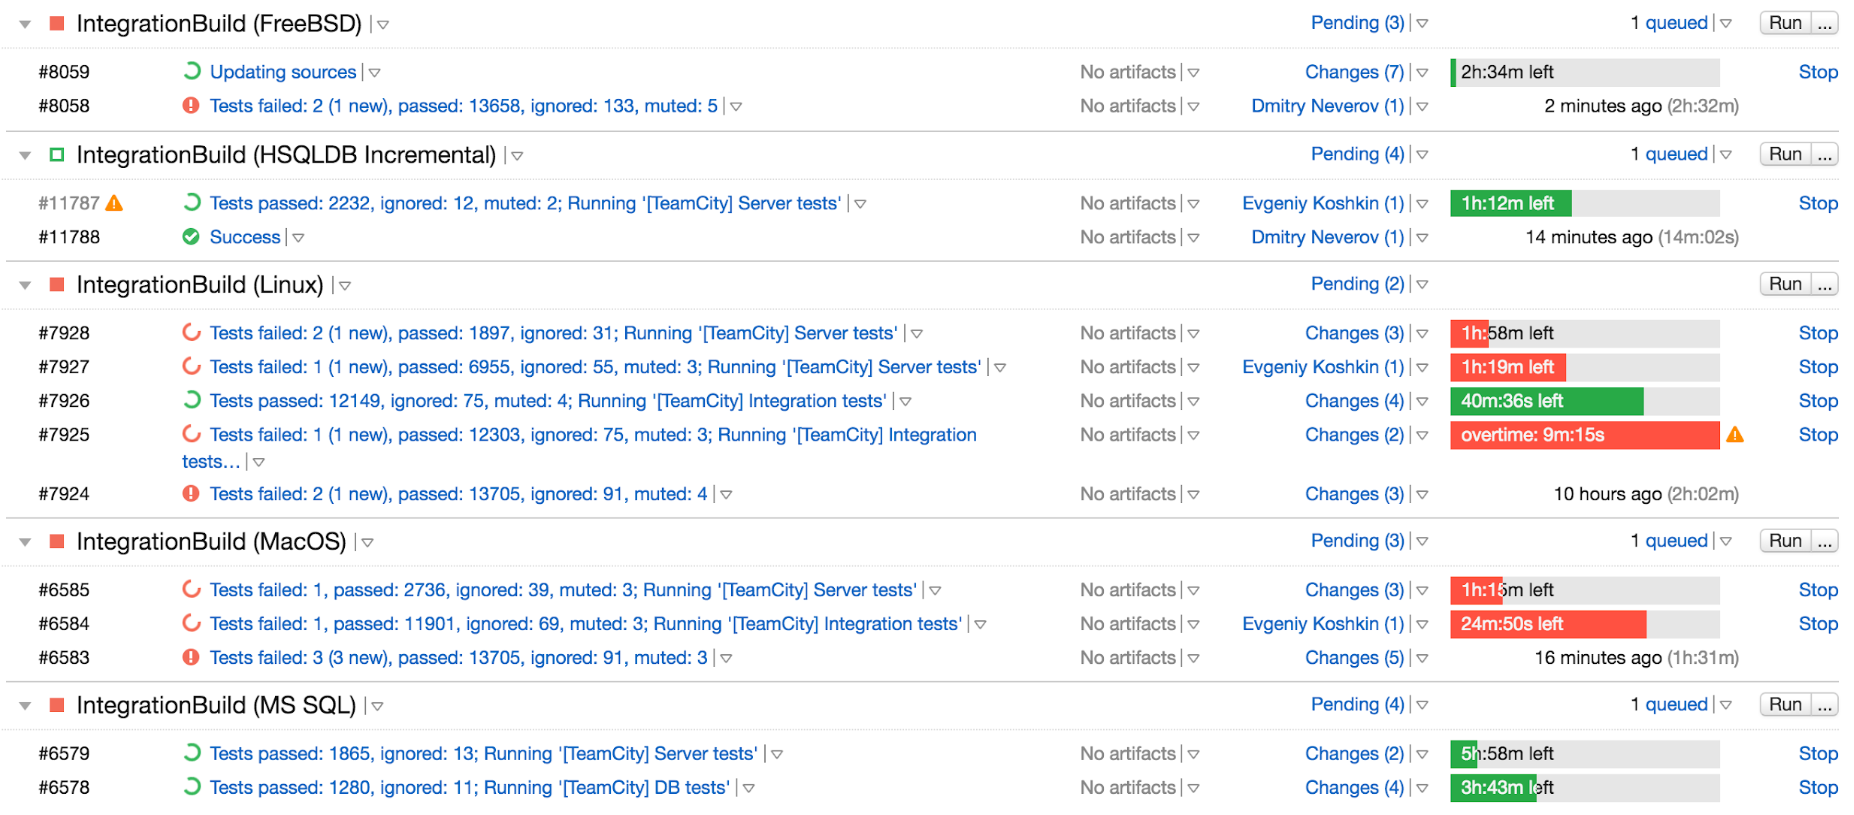
\includegraphics[width=\textwidth]{teamCity.png}
        \end{center}
    \end{frame}

    \begin{frame}
        \frametitle{Jenkins}
        \begin{center}
            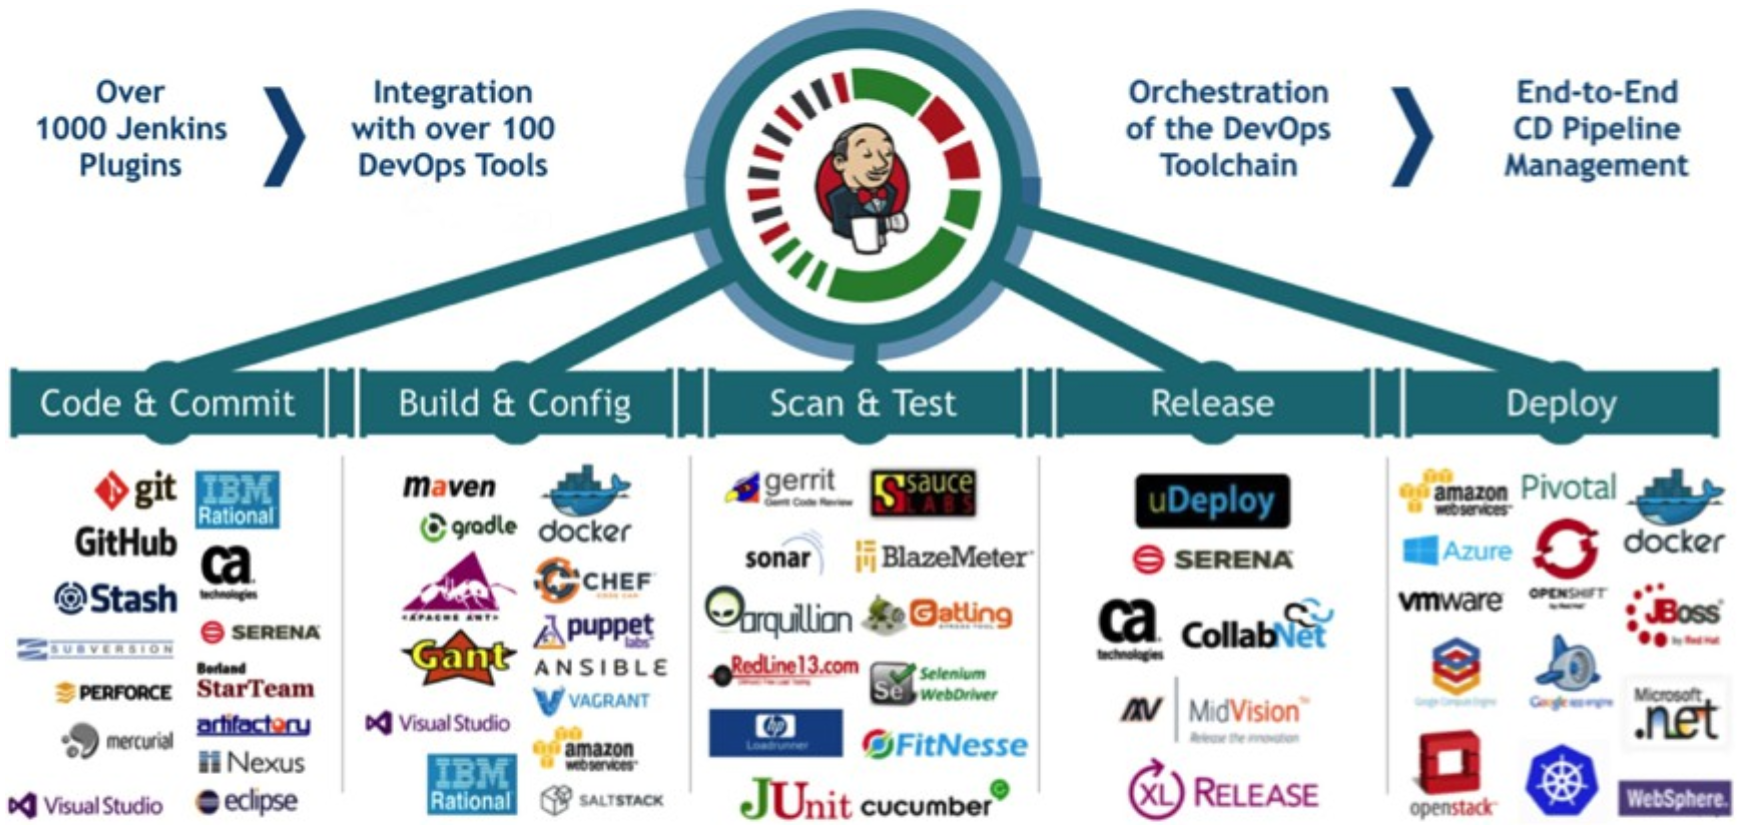
\includegraphics[width=\textwidth]{jenkins.png}
        \end{center}
    \end{frame}

    \begin{frame}
        \frametitle{Continuous Integration: полезные практики}
        \begin{outline}
            \1 Не коммитим в сломанный билд
            \1 Проверяем все тесты локально перед коммитом
                \2 Проверяем мердж мастера в локальную ветку (если работаем с веткой)
                \2 pre-tested commits
            \1 Ждём результата сборки на сервере перед новой задачей
            \1 Сломанному билду нет оправданий
                \2 Кто сломал, тот и виноват
                \2 Всегда будь готов откатить изменения
                \2 Временной лимит на починку билда
            \1 Настраиваем систему оповещений
        \end{outline}
    \end{frame}

    \section{Конвейер сборки}

    \begin{frame}
        \begin{center}
            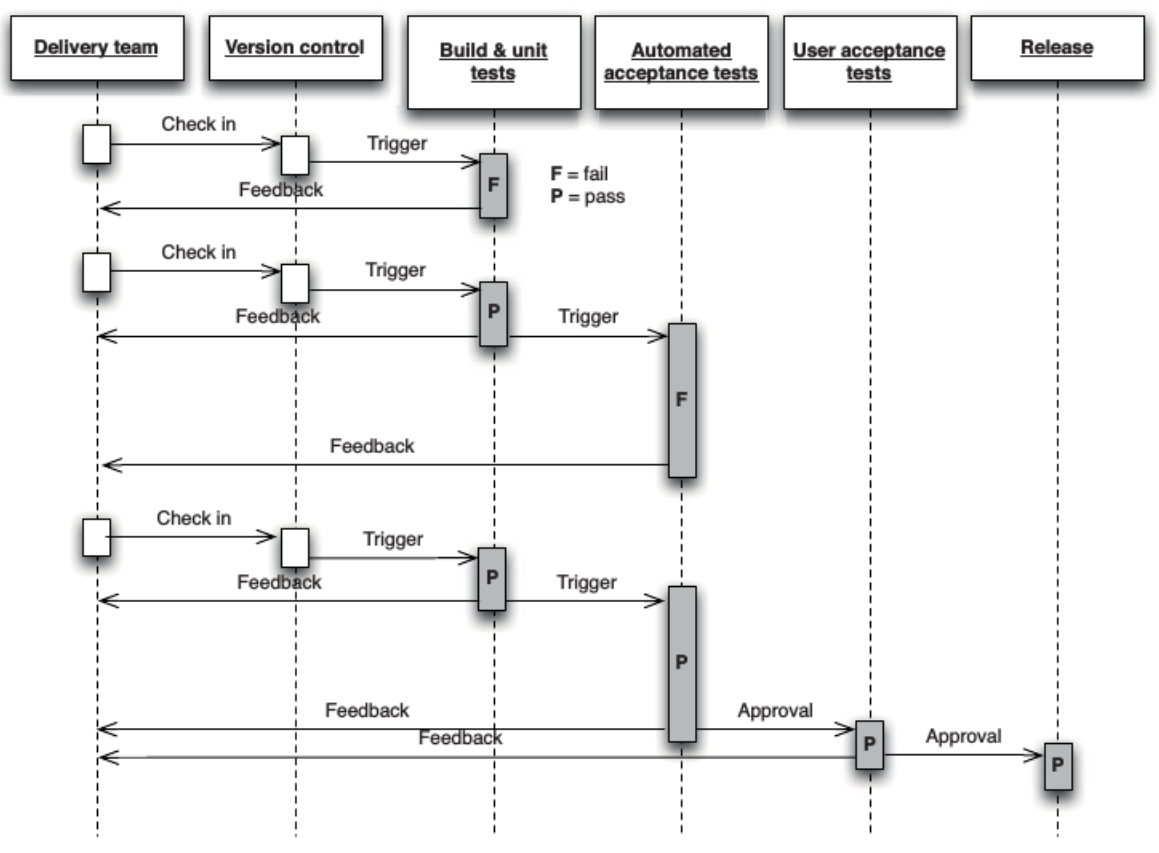
\includegraphics[width=0.95\textwidth]{cdPipeline.png}
        \end{center}
    \end{frame}

    \begin{frame}
        \begin{center}
            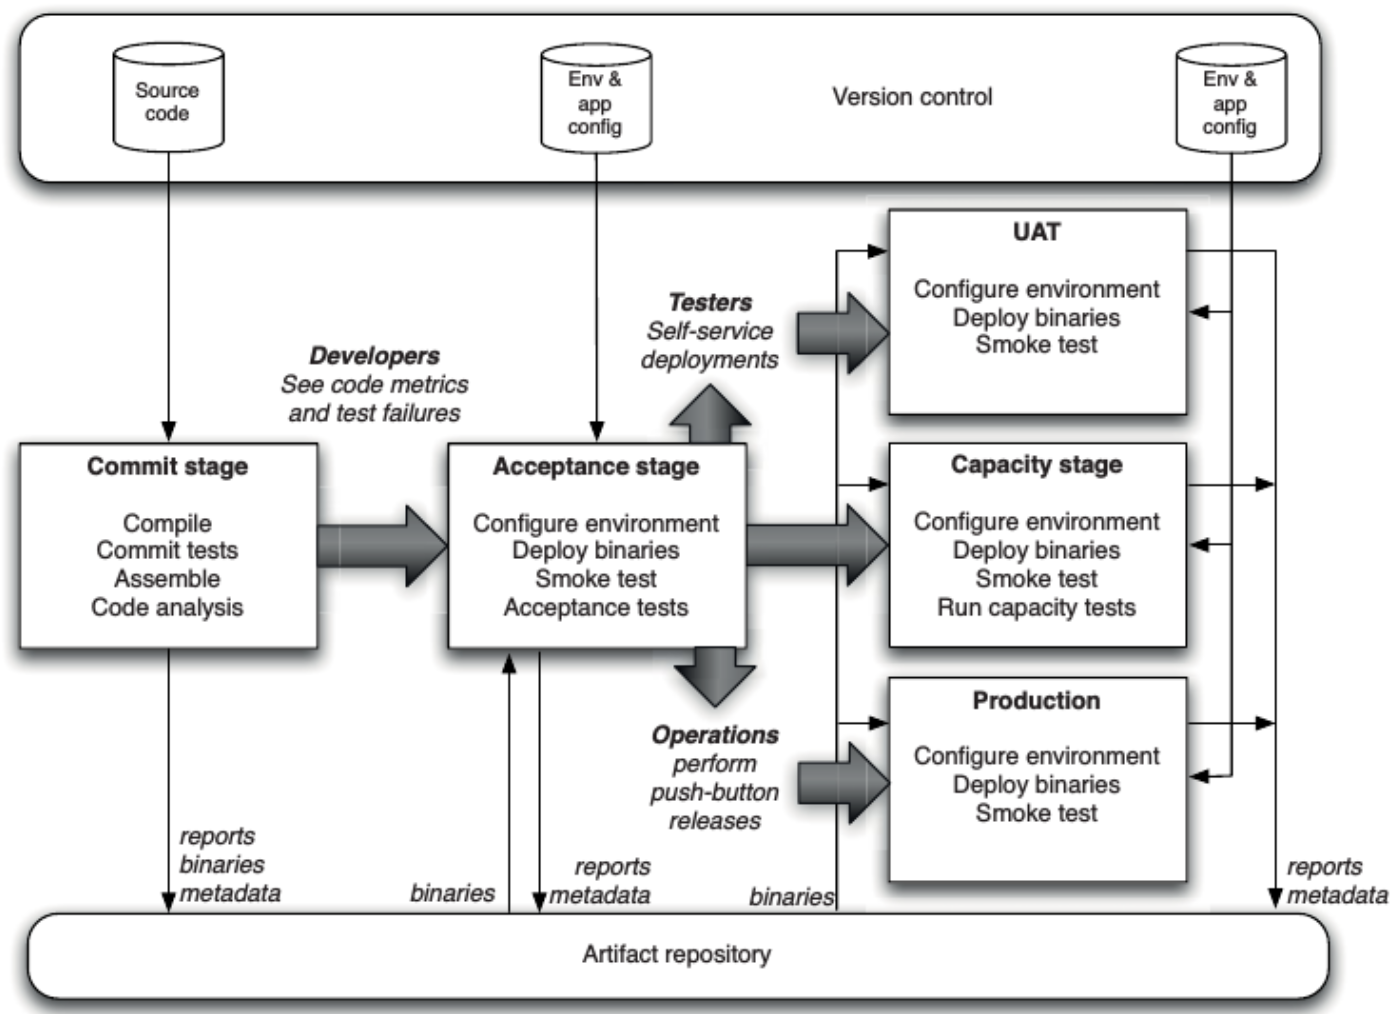
\includegraphics[width=0.95\textwidth]{cdStages.png}
        \end{center}
    \end{frame}

    \begin{frame}
        \frametitle{Ещё полезные практики}
        \begin{outline}
            \1 Собираем бинарники только один раз
                \2 Кэширование запусков конвейера
            \1 Один и тот же процесс развёртывания для разных окружений
                \2 Отделение кода от конфигурации окружения
            \1 Запуск smoke test’ов после развёртывания
            \1 Развёртывание в копии production окружения
        \end{outline}
    \end{frame}

    \begin{frame}
        \frametitle{Ещё полезные практики}
        \begin{outline}[enumerate]
            \1 Проектирование основных этапов и создание скелета
            \1 Автоматизирование сборки и развёртывания
            \1 Автоматизирование модульных тестов и анализа кода
            \1 Автоматизирование приёмочных тестов
            \1 Эволюционирование конвейера
        \end{outline}
    \end{frame}

    \begin{frame}
        \frametitle{Модель зрелости процесса управления релизами}
        \begin{center}
            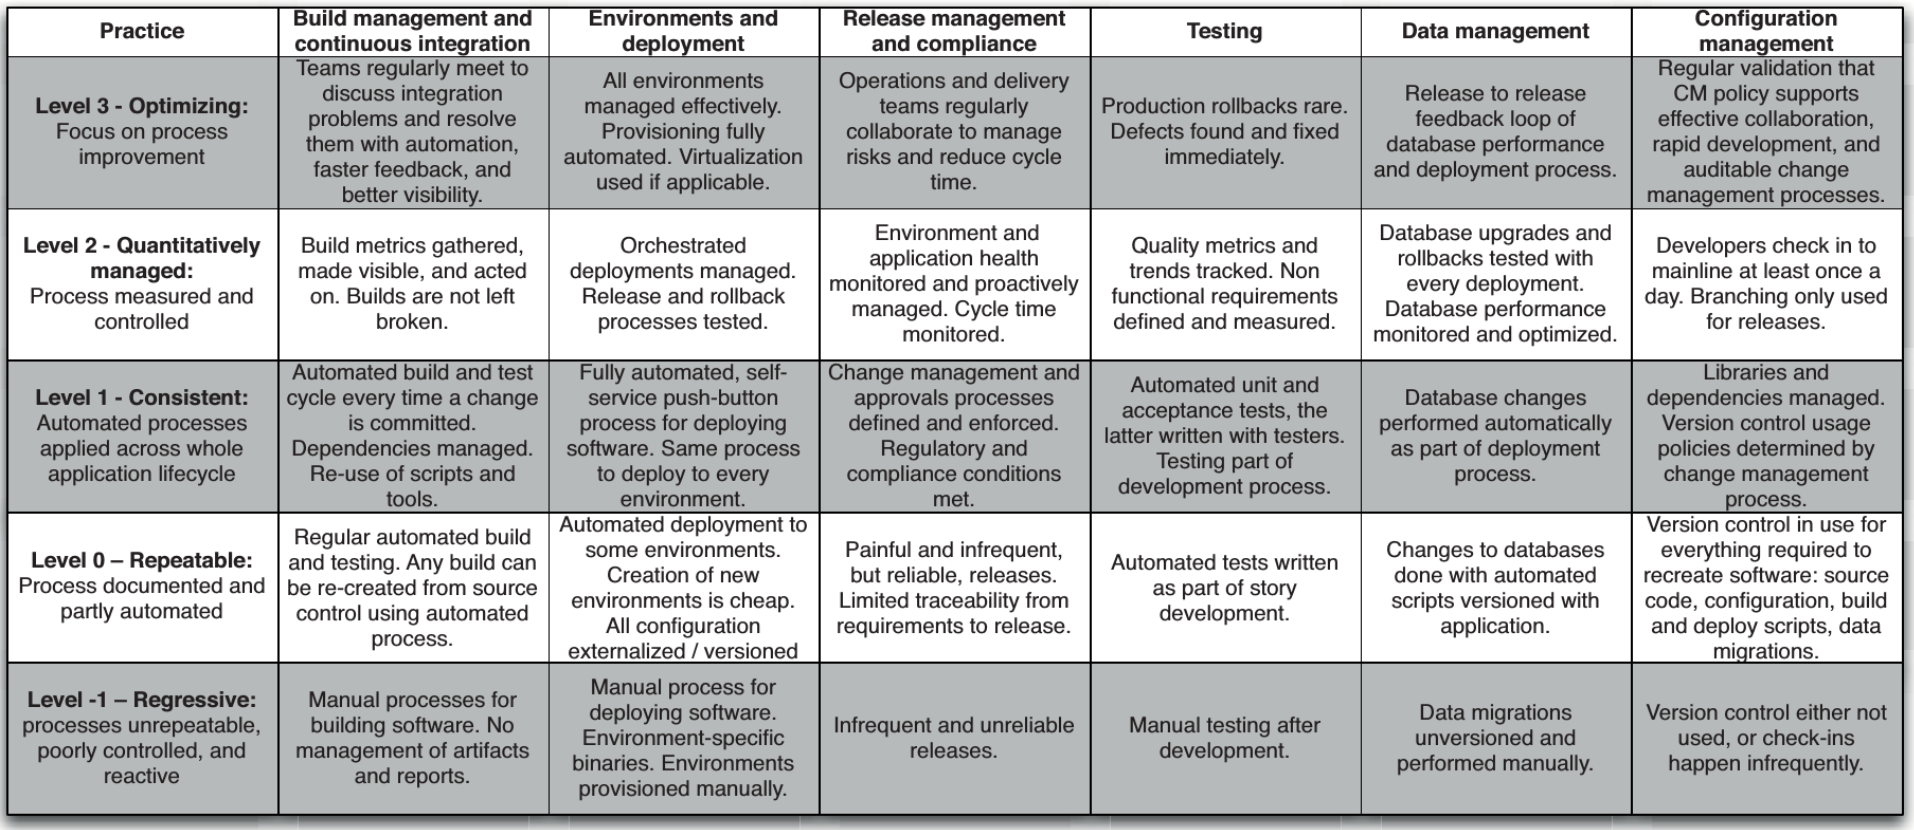
\includegraphics[width=\textwidth]{cdMaturityModel.png}
        \end{center}
    \end{frame}

    \begin{frame}
        \frametitle{Что почитать}
        \begin{center}
            
\includegraphics[width=\textwidth]{books.png}
        \end{center}
    \end{frame}

\end{document}